\documentclass[11pt,a4paper]{article}


%%% packages

  \usepackage{a4wide, tikz}


%%% TikZ

  \usetikzlibrary{calc}
  \tikzset{ v/.style = { circle
                       , draw
                       , thick
                       , inner sep    = 0.5pt
                       , minimum size = 6.0mm
                       },
            t/.style = { circle
            , draw = black
            , thick
            , inner sep    = 0.5pt
            , minimum size = 6.0mm
            }
          }



%%% front matter

  \title{Coursework 3: Graph Algorithms and Complexity Theory}
  \author{Oskar Mampe}
  \date{Tutorial Session: Thursday 1pm}

\begin{document}

\maketitle
\thispagestyle{empty}
%%%%%%%%%%%%%%%%%%%%%%%%%%%% ORIGINAL %%%%%%%%%%%%%%%%%%%%%%%%%%%% 
\noindent In the graph below a matching is indicated by bold lines. The trees created will also have a bold line indicating a matching.

\begin{center}
  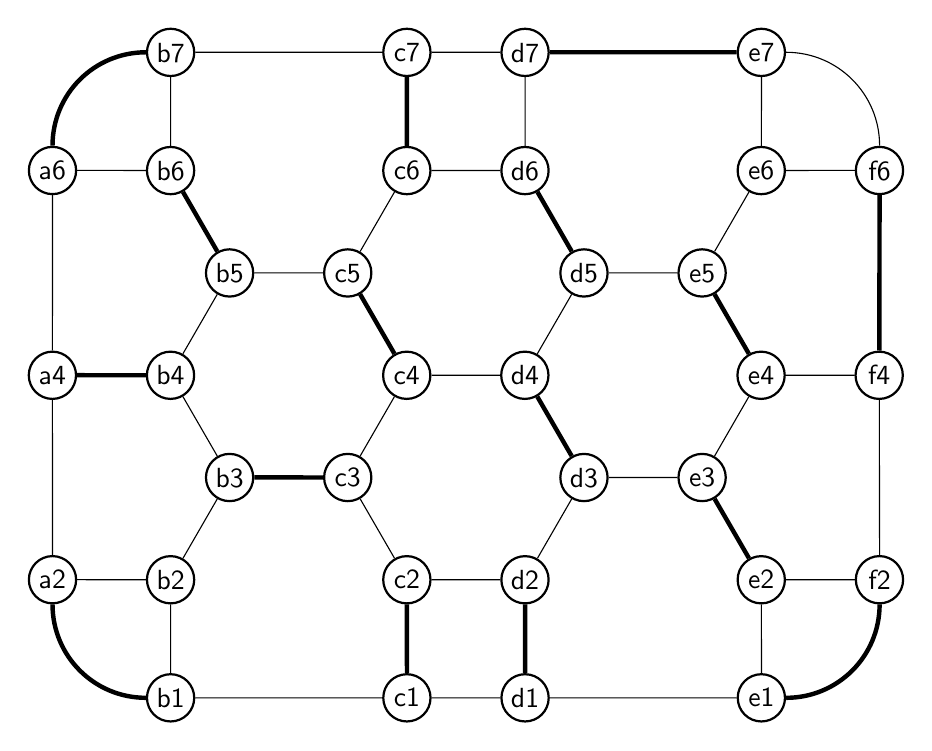
\begin{tikzpicture}[scale=1.5, bend angle=45, font=\sffamily]
    \foreach \n/\x in {a/1, b/2, c/4, d/5, e/7,f/8} {
      \node[v] (\n4) at (\x,4) {\n4};
    }
    \foreach \n in {b,d} {
      \node[v] (\n3) at ($(\n4) + (300:1)$) {\n3};
      \node[v] (\n5) at ($(\n4) + ( 60:1)$) {\n5};
      \node[v] (\n2) at ($(\n3) + (240:1)$) {\n2};
      \node[v] (\n6) at ($(\n5) + (120:1)$) {\n6};
      \node[v] (\n1) at ($(\n2) + (270:1)$) {\n1};
      \node[v] (\n7) at ($(\n6) + ( 90:1)$) {\n7};
    }
    \foreach \n in {c,e} {
      \node[v] (\n3) at ($(\n4) + (240:1)$) {\n3};
      \node[v] (\n5) at ($(\n4) + (120:1)$) {\n5};
      \node[v] (\n2) at ($(\n3) + (300:1)$) {\n2};
      \node[v] (\n6) at ($(\n5) + ( 60:1)$) {\n6};
      \node[v] (\n1) at ($(\n2) + (270:1)$) {\n1};
      \node[v] (\n7) at ($(\n6) + ( 90:1)$) {\n7};
    }
    \foreach \h in {2,6} {
      \node[v] (a\h) at ($(b\h) + (180:1)$) {a\h};
      \node[v] (f\h) at ($(e\h) + (  0:1)$) {f\h};
    }
    \draw[ultra thick] (a2) to[bend right] (b1)
                       (e1) to[bend right] (f2)
                       (b7) to[bend right] (a6);
    \draw[ultra thick] (c1)--(c2)  (d1)--(d2)  (b3)--(c3)  (e2)--(e3)
           (a4)--(b4)  (c4)--(c5)  (d3)--(d4)  (e4)--(e5)  (f4)--(f6)
           (b5)--(b6)  (c6)--(c7)  (d5)--(d6)  (d7)--(e7);
    \draw (f6) to[bend right] (e7);
    \draw (b2)--(b3)--(b4)--(b5)--(c5)--(c6)--(d6)--(d7)--(c7)--(b7)--(b6)
        --(a6)--(a4)--(a2)--(b2)--(b1)--(c1)--(d1)--(e1)--(e2)--(f2)--(f4)
        --(e4)--(e3)--(d3)--(d2)--(c2)--(c3)--(c4)--(d4)--(d5)--(e5)--(e6)
        --(f6)  (e6)--(e7);
  \end{tikzpicture}
\end{center}


\vspace{\fill}

There are two M-unsaturated vertices, namely b2 and e6. Therefore, I initiate Edmond's algorithm starting by growing two alternative trees starting at these two vertices.

%%%%%%%%%%%%%%%%%%%%%%%%%%%% FIRST PASS %%%%%%%%%%%%%%%%%%%%%%%%%%%%
\begin{center}
    \begin{minipage}{.6\textwidth}
        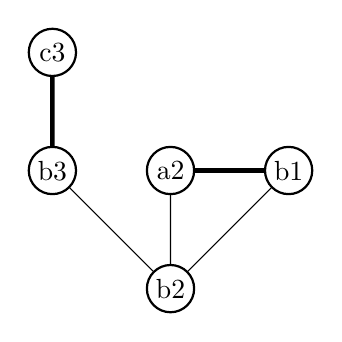
\begin{tikzpicture}
            \node[t]  {b2} [grow=up]
            %[sibling distance=0.7cm,level distance = 1.4cm,red]
            child[draw=black, thin] { 
                node[t] (b1) {b1}
            }
            child [draw=black, thin] {
                node[t] (a2) {a2}
            }
            child [draw=black, thin] {
                node[t] {b3}
                child[draw=black, ultra thick] {
                    node[t] {c3}
                }
            };
            \path[draw=black,ultra thick] (b1) edge(a2);
            \end{tikzpicture}

    \end{minipage}
    \begin{minipage}{.2\textwidth}
        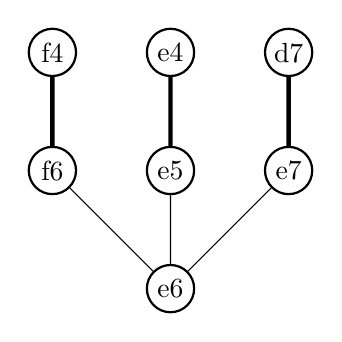
\begin{tikzpicture}
            \node[t]  {e6} [grow=up]
            %[sibling distance=0.7cm,level distance = 1.4cm,red]
            child[draw=black, thin] { 
                node[t] (e7) {e7}
                child[draw=black, ultra thick] {
                    node[t] {d7}
                }
            }
            child [draw=black, thin] {
                node[t] (e5) {e5}
                child[draw=black, ultra thick] {
                    node[t] {e4}
                }
            }
            child [draw=black, thin] {
                node[t] {f6}
                child[draw=black, ultra thick] {
                    node[t] {f4}
                }
            };
        \end{tikzpicture}
    \end{minipage}
\end{center}

A blossom has been found. The blossom consists of vertices b2, a2, b1 and I shrink it to vertex $\alpha$.
This way, I obtain the following graph:

\begin{center}
    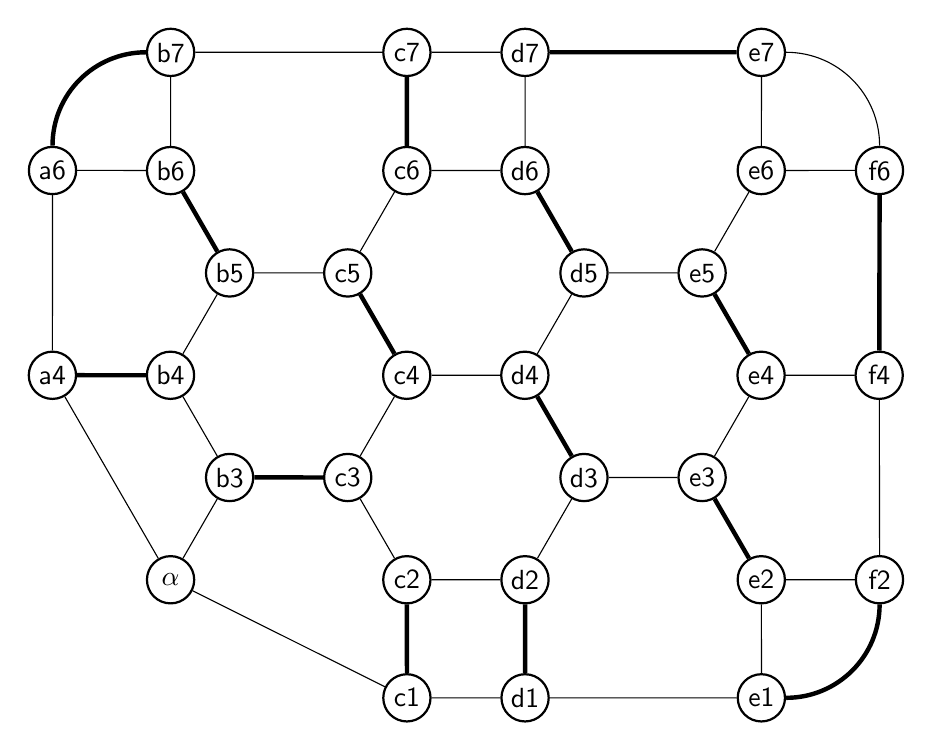
\begin{tikzpicture}[scale=1.5, bend angle=45, font=\sffamily]
      %\foreach \n/\x in {a/1, b/2, c/4, d/5, e/7,f/8} {
       \node[v] (a4) at (1,4) {a4};
       \node[v] (b4) at (2,4) {b4};
       \node[v] (c4) at (4,4) {c4};
       \node[v] (d4) at (5,4) {d4};
       \node[v] (e4) at (7,4) {e4};
       \node[v] (f4) at (8,4) {f4};
      %}
      %\foreach \n in {b,d} {
        \node[v] (b3) at ($(b4) + (300:1)$) {b3};
        \node[v] (b5) at ($(b4) + ( 60:1)$) {b5};
        \node[v] (alpha) at ($(b3) + (240:1)$) {$\alpha$};
        \node[v] (b6) at ($(b5) + (120:1)$) {b6};
        \node[v] (b7) at ($(b6) + ( 90:1)$) {b7};

        \node[v] (d3) at ($(d4) + (300:1)$) {d3};
        \node[v] (d5) at ($(d4) + ( 60:1)$) {d5};
        \node[v] (d2) at ($(d3) + (240:1)$) {d2};
        \node[v] (d6) at ($(d5) + (120:1)$) {d6};
        \node[v] (d1) at ($(d2) + (270:1)$) {d1};
        \node[v] (d7) at ($(d6) + ( 90:1)$) {d7};
      %}
      %\foreach \n in {c,e} {
        \node[v] (c3) at ($(c4) + (240:1)$) {c3};
        \node[v] (c5) at ($(c4) + (120:1)$) {c5};
        \node[v] (c2) at ($(c3) + (300:1)$) {c2};
        \node[v] (c6) at ($(c5) + ( 60:1)$) {c6};
        \node[v] (c1) at ($(c2) + (270:1)$) {c1};
        \node[v] (c7) at ($(c6) + ( 90:1)$) {c7};

        \node[v] (e3) at ($(e4) + (240:1)$) {e3};
        \node[v] (e5) at ($(e4) + (120:1)$) {e5};
        \node[v] (e2) at ($(e3) + (300:1)$) {e2};
        \node[v] (e6) at ($(e5) + ( 60:1)$) {e6};
        \node[v] (e1) at ($(e2) + (270:1)$) {e1};
        \node[v] (e7) at ($(e6) + ( 90:1)$) {e7};
      %}
      %\foreach \h in {2,6} {
        \node[v] (f2) at ($(e2) + (  0:1)$) {f2};

        \node[v] (a6) at ($(b6) + (180:1)$) {a6};
        \node[v] (f6) at ($(e6) + (  0:1)$) {f6};
      %}
      \draw[ultra thick] (e1) to[bend right] (f2)
                         (b7) to[bend right] (a6);
      \draw[ultra thick] (c1)--(c2)  (d1)--(d2)  (b3)--(c3)  (e2)--(e3)
             (a4)--(b4)  (c4)--(c5)  (d3)--(d4)  (e4)--(e5)  (f4)--(f6)
             (b5)--(b6)  (c6)--(c7)  (d5)--(d6)  (d7)--(e7);
      \draw (f6) to[bend right] (e7);
      \draw (alpha)--(b3)--(b4)--(b5)--(c5)--(c6)--(d6)--(d7)--(c7)--(b7)--(b6)
          --(a6)--(a4)--(alpha)--(c1)--(d1)--(e1)--(e2)--(f2)--(f4)
          --(e4)--(e3)--(d3)--(d2)--(c2)--(c3)--(c4)--(d4)--(d5)--(e5)--(e6)
          --(f6)  (e6)--(e7);
    \end{tikzpicture}
  \end{center}

%%%%%%%%%%%%%%%%%%%%%%%%%%%% SECOND PASS %%%%%%%%%%%%%%%%%%%%%%%%%%%%
$\alpha$ and e6 are M-unsaturated, so I start growing the two alternative trees again.
  \begin{center}
    \begin{minipage}{.6\textwidth}
        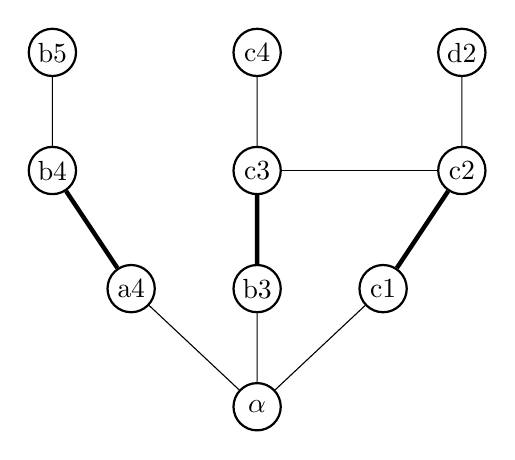
\begin{tikzpicture}[level distance=15mm,
            level 1/.style={sibling distance=8mm},
            level 2/.style={sibling distance=20mm},
            level 3/.style={sibling distance=15mm}]
            \node[t]  {$\alpha$} [grow=up]
            %[sibling distance=0.7cm,level distance = 1.4cm,red]
            child [draw=black, thin] {
                node[t] (c1) {c1}
                child[draw=black, ultra thick] {
                    node[t] (c2) {c2}
                    child[draw=black, thin] { 
                        node[t] (d2) {d2}
                    }
                }
                child[missing]
            }
            child[missing]
            child [draw=black, thin] {
                node[t] (b3) {b3}
                child[draw=black, ultra thick] {
                    node[t] (c3) {c3}
                    child[draw=black, thin] { 
                        node[t] (c4) {c4}
                    }
                }
            }
            child[missing]
            child[draw=black, thin] { 
                node[t] (a4) {a4}
                child[missing]
                child[draw=black, ultra thick] {
                    node[t] (b4) {b4}
                    child[draw=black, thin] { 
                        node[t] (b5) {b5}
                    }
                }
            };
            %\path[draw=black,thin] (b4) edge(b3);
            \path[draw=black,thin] (c2) edge(c3);
            \end{tikzpicture}

    \end{minipage}
    \begin{minipage}{.1\textwidth}
        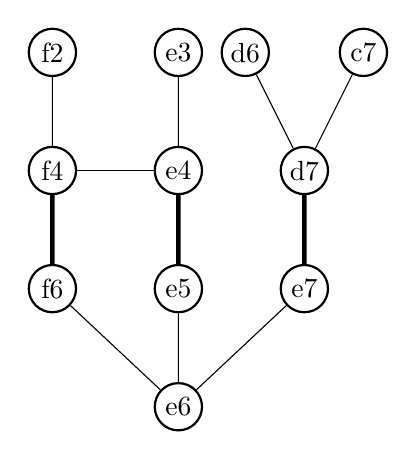
\begin{tikzpicture}[level distance=15mm,
            level 1/.style={sibling distance=8mm},
            level 2/.style={sibling distance=20mm},
            level 3/.style={sibling distance=15mm}]
            \node[t]  {e6} [grow=up]
            %[sibling distance=0.7cm,level distance = 1.4cm,red]
            child[draw=black, thin] { 
                node[t] (e7) {e7}
                child[draw=black, ultra thick] {
                    node[t] {d7}
                    child[draw=black, thin] {
                        node[t] {c7}
                    }
                    child[draw=black, thin] {
                        node[t] {d6}
                    }
                }
            }
            child[missing]
            child [draw=black, thin] {
                node[t] (e5) {e5}
                child[draw=black, ultra thick] {
                    node[t] (e4) {e4}
                    child[draw=black, thin] {
                        node[t] (e3) {e3}
                    }
                }
            }
            child[missing]
            child [draw=black, thin] {
                node[t] {f6}
                child[draw=black, ultra thick] {
                    node[t] (f4) {f4}
                    child[draw=black, thin] {
                        node[t] {f2}
                    }
                }
            };
            \path[draw=black,thin] (e4) edge(f4);
        \end{tikzpicture}
    \end{minipage}
\end{center}

Another two blossoms have been found. One of them being containing $\alpha$, b3,  c3, c2, c1 I will shrink this to vertex $\beta$.
The other blossom consists of e6, e5, e4, f4, f6 I will shrink this to vertex $\gamma$. The following graph is obtained:
\hspace{\fill}


\begin{center}
    \begin{tikzpicture}[scale=1.5, bend angle=45, font=\sffamily]
      %\foreach \n/\x in {a/1, b/2, c/4, d/5, e/7,f/8} {
        \node[v] (a4) at (1,4) {a4};
        \node[v] (b4) at (2,4) {b4};
        \node[v] (c4) at (4,4) {c4};
        \node[v] (d4) at (5,4) {d4};
        \node[draw=none] (e4) at (7,4) {};
        \node[draw=none] (f4) at (8,4) {};
       %}
       %\foreach \n in {b,d} {
         \node[draw=none] (b3) at ($(b4) + (300:1)$) {};
         \node[v] (b5) at ($(b4) + ( 60:1)$) {b5};
         \node[v] (beta) at ($(b3) + (240:1)$) {$\beta$};
         \node[v] (b6) at ($(b5) + (120:1)$) {b6};
         \node[v] (b7) at ($(b6) + ( 90:1)$) {b7};
 
         \node[v] (d3) at ($(d4) + (300:1)$) {d3};
         \node[v] (d5) at ($(d4) + ( 60:1)$) {d5};
         \node[v] (d2) at ($(d3) + (240:1)$) {d2};
         \node[v] (d6) at ($(d5) + (120:1)$) {d6};
         \node[v] (d1) at ($(d2) + (270:1)$) {d1};
         \node[v] (d7) at ($(d6) + ( 90:1)$) {d7};
       %}
       %\foreach \n in {c,e} {
         \node[draw=none] (c3) at ($(c4) + (240:1)$) {};
         \node[v] (c5) at ($(c4) + (120:1)$) {c5};
         \node[draw=none] (c2) at ($(c3) + (300:1)$) {};
         \node[v] (c6) at ($(c5) + ( 60:1)$) {c6};
         \node[draw=none] (c1) at ($(c2) + (270:1)$) {};
         \node[v] (c7) at ($(c6) + ( 90:1)$) {c7};
 
         \node[v] (e3) at ($(e4) + (240:1)$) {e3};
         \node[draw=none] (e5) at ($(e4) + (120:1)$) {};
         \node[v] (e2) at ($(e3) + (300:1)$) {e2};
         \node[v] (gamma) at ($(e5) + ( 60:1)$) {$\gamma$};
         \node[v] (e1) at ($(e2) + (270:1)$) {e1};
         \node[v] (e7) at ($(e6) + ( 90:1)$) {e7};
       %}
       %\foreach \h in {2,6} {
         \node[v] (f2) at ($(e2) + (  0:1)$) {f2};
 
         \node[v] (a6) at ($(b6) + (180:1)$) {a6};
         \node[draw=none] (f6) at ($(e6) + (  0:1)$) {};
      %}
      \draw[ultra thick] (e1) to[bend right] (f2)
                         (b7) to[bend right] (a6);
      \draw[ultra thick]  (d1)--(d2)  (e2)--(e3) (a4)--(b4)  
             (c4)--(c5)  (d3)--(d4)
             (b5)--(b6)  (c6)--(c7)  (d5)--(d6)  (d7)--(e7);
      \draw (beta)--(b4)--(b5)--(c5)--(c6)--(d6)--(d7)--(c7)--(b7)--(b6)
          --(a6)--(a4)--(beta)--(d1)--(e1)--(e2)--(f2)--(gamma)
          --(e3)--(d3)--(d2)--(beta)--(c4)--(d4)--(d5)--(gamma)
            (gamma)--(e7);
    \end{tikzpicture}
  \end{center}

  %%%%%%%%%%%%%%%%%%%%%%%%%%%% THIRD PASS %%%%%%%%%%%%%%%%%%%%%%%%%%%%

  The two M-unsaturated vertices left are $\beta$ and $\gamma$. Therefore, the following alternative trees are grown:

  \begin{center}
    \begin{minipage}{.6\textwidth}
        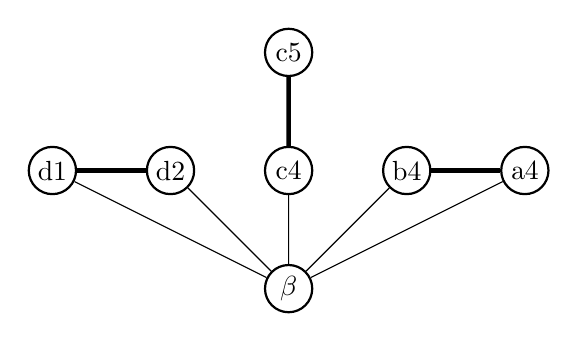
\begin{tikzpicture}
            \node[t]  {$\beta$} [grow=up]
            %[sibling distance=0.7cm,level distance = 1.4cm,red]
            child[draw=black, thin] { 
                node[t] (a4) {a4}
            }
            child [draw=black, thin] {
                node[t] (b4) {b4}
            }
            child [draw=black, thin] {
                node[t] (c4) {c4}
                child[draw=black, ultra thick] {
                    node[t] {c5}
                }
            }
            child [draw=black, thin] {
                node[t] (d2) {d2}
            }
            child [draw=black, thin] {
                node[t] (d1) {d1}
            };
            \path[draw=black,ultra thick] (a4) edge(b4);
            \path[draw=black,ultra thick] (d1) edge(d2);
            \end{tikzpicture}

    \end{minipage}
    \begin{minipage}{.1\textwidth}
        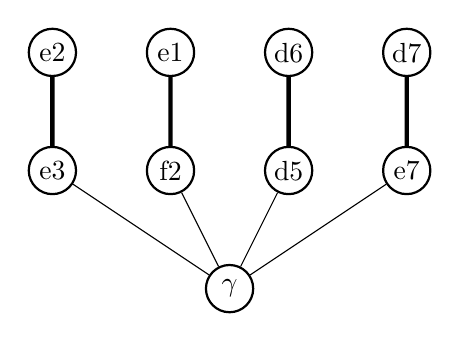
\begin{tikzpicture}
            \node[t]  {$\gamma$} [grow=up]
            %[sibling distance=0.7cm,level distance = 1.4cm,red]
            child[draw=black, thin] { 
                node[t] (e7) {e7}
                child[draw=black, ultra thick] {
                    node[t] {d7}
                }
            }
            child [draw=black, thin] {
                node[t] (d5) {d5}
                child[draw=black, ultra thick] {
                    node[t] {d6}
                }
            }
            child [draw=black, thin] {
                node[t] (f2) {f2}
                child[draw=black, ultra thick] {
                    node[t] {e1}
                }
            }
            child [draw=black, thin] {
                node[t] {e3}
                child[draw=black, ultra thick] {
                    node[t] {e2}
                }
            };
        \end{tikzpicture}
    \end{minipage}

    I have found two blossoms. One of them being $\beta$, d1, d2 and the other $\beta$, b4, a4.
    Both of these can be shrunk to a single vertex $\delta$. The following graph is then produced:

    \begin{center}
        \begin{tikzpicture}[scale=1.5, bend angle=45, font=\sffamily]
          %\foreach \n/\x in {a/1, b/2, c/4, d/5, e/7,f/8} {
            \node[draw=none] (a4) at (1,4) {};
            \node[draw=none] (b4) at (2,4) {};
            \node[v] (c4) at (4,4) {c4};
            \node[v] (d4) at (5,4) {d4};
            \node[draw=none] (e4) at (7,4) {};
            \node[draw=none] (f4) at (8,4) {};
           %}
           %\foreach \n in {b,d} {
             \node[draw=none] (b3) at ($(b4) + (300:1)$) {};
             \node[v] (b5) at ($(b4) + ( 60:1)$) {b5};
             \node[v] (delta) at ($(b3) + (240:1)$) {$\delta$};
             \node[v] (b6) at ($(b5) + (120:1)$) {b6};
             \node[v] (b7) at ($(b6) + ( 90:1)$) {b7};
     
             \node[v] (d3) at ($(d4) + (300:1)$) {d3};
             \node[v] (d5) at ($(d4) + ( 60:1)$) {d5};
             \node[draw=none] (d2) at ($(d3) + (240:1)$) {};
             \node[v] (d6) at ($(d5) + (120:1)$) {d6};
             \node[draw=none] (d1) at ($(d2) + (270:1)$) {};
             \node[v] (d7) at ($(d6) + ( 90:1)$) {d7};
           %}
           %\foreach \n in {c,e} {
             \node[draw=none] (c3) at ($(c4) + (240:1)$) {};
             \node[v] (c5) at ($(c4) + (120:1)$) {c5};
             \node[draw=none] (c2) at ($(c3) + (300:1)$) {};
             \node[v] (c6) at ($(c5) + ( 60:1)$) {c6};
             \node[draw=none] (c1) at ($(c2) + (270:1)$) {};
             \node[v] (c7) at ($(c6) + ( 90:1)$) {c7};
     
             \node[v] (e3) at ($(e4) + (240:1)$) {e3};
             \node[draw=none] (e5) at ($(e4) + (120:1)$) {};
             \node[v] (e2) at ($(e3) + (300:1)$) {e2};
             \node[v] (gamma) at ($(e5) + ( 60:1)$) {$\gamma$};
             \node[v] (e1) at ($(e2) + (270:1)$) {e1};
             \node[v] (e7) at ($(e6) + ( 90:1)$) {e7};
           %}
           %\foreach \h in {2,6} {
             \node[v] (f2) at ($(e2) + (  0:1)$) {f2};
     
             \node[v] (a6) at ($(b6) + (180:1)$) {a6};
             \node[draw=none] (f6) at ($(e6) + (  0:1)$) {};
          %}
          \draw[ultra thick] (e1) to[bend right] (f2)
                             (b7) to[bend right] (a6);
          \draw[ultra thick]   (e2)--(e3)
                 (c4)--(c5)  (d3)--(d4)
                 (b5)--(b6)  (c6)--(c7)  (d5)--(d6)  (d7)--(e7);
          \draw (delta)--(b5)--(c5)--(c6)--(d6)--(d7)--(c7)--(b7)--(b6)
              --(a6)--(delta)--(e1)--(e2)--(f2)--(gamma)
              --(e3)--(d3)--(delta)--(c4)--(d4)--(d5)--(gamma)
                (gamma)--(e7);
        \end{tikzpicture}
      \end{center} 

      The two M-unsaturated vertices are $\delta$ and $\gamma$ so the two alternative trees are created:

      \begin{center}
        \begin{minipage}{.6\textwidth}
            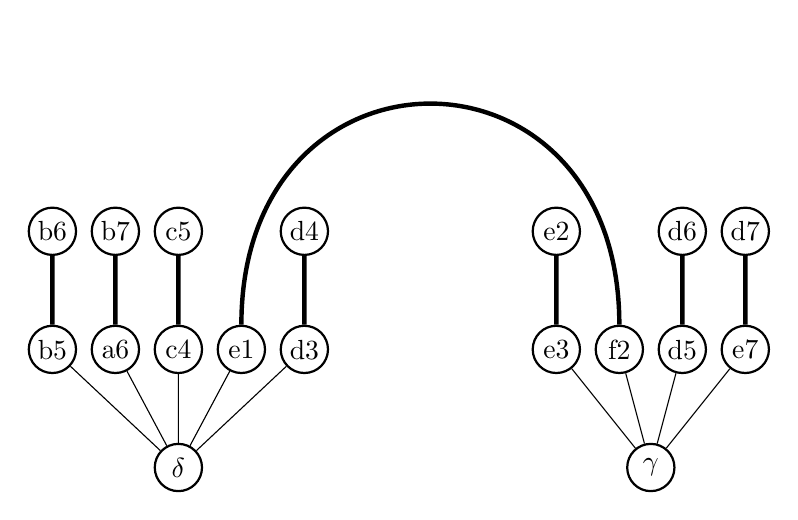
\begin{tikzpicture}[level distance=15mm,
            level 1/.style={sibling distance=8mm},
            level 2/.style={sibling distance=20mm},
            level 3/.style={sibling distance=15mm}]
                \node[t]  {$\delta$} [grow=up, sibling distance=0.7cm]
                %[sibling distance=0.7cm,level distance = 1.4cm,red]
                child [draw=black, thin] {
                    node[t] (d3) {d3}
                    child[draw=black, ultra thick] {
                        node[t] {d4}
                    }
                }
                child [draw=black, thin] {
                    node[t] (e1) {e1}
                }
                child [draw=black, thin] {
                    node[t] (c4) {c4}
                    child[draw=black, ultra thick] {
                        node[t] {c5}
                    }
                }
                child [draw=black, thin] {
                    node[t] (a6) {a6}
                    child[draw=black, ultra thick] {
                        node[t] {b7}
                    }
                }
                child [draw=black, thin] {
                    node[t] (b5) {b5}
                    child[draw=black, ultra thick] {
                        node[t] {b6}
                    }
                };
                \begin{scope}[xshift=6cm]
                \node[t]  {$\gamma$} [grow=up]
                %[sibling distance=0.7cm,level distance = 1.4cm,red]
                child[draw=black, thin] { 
                    node[t] (e7) {e7}
                    child[draw=black, ultra thick] {
                        node[t] {d7}
                    }
                }
                child [draw=black, thin] {
                    node[t] (d5) {d5}
                    child[draw=black, ultra thick] {
                        node[t] {d6}
                    }
                }
                child [draw=black, thin] {
                    node[t] (f2) {f2}
                }
                child [draw=black, thin] {
                    node[t] {e3}
                    child[draw=black, ultra thick] {
                        node[t] {e2}
                    }
                };
                \draw[black, ultra thick] (e1) to[bend left=90, looseness=2] (f2);
                %\draw [->] (J) to [out=0,in=-90] ($(I)+(1,0)$) to [out=90, in=0 ] (B);
                \end{scope}
            \end{tikzpicture}
        \end{minipage}
    \end{center}

    An augmenting path has been found. The path being ($\delta$, e1, f2, $\gamma$). This can be further simplified, by first going around the first blossom \{$\beta$, d2, d1\} and the second blossom \{f4, f6, e6\}, making the augmenting path ($\beta$, d2, d1, e1, f2, f4, f6, e6). There is another blossom to traverse, for which I have chosen the path \{$\alpha$, c1, c2\} as it is the only alternative path do d2. This makes the path now ($\alpha$, c1, c2, d2, d1, e1, f2, f4, f6, e6). Finally, I traverse the last blossom \{b2, a2, b1\} as it is the only alternative path to c1. Making the final path (b2, a2, b1, c1, c2, d2, d1, e1, f2, f4, f6, e6). I augment the mathicng along the path, and find this following matching:
    \begin{center}
        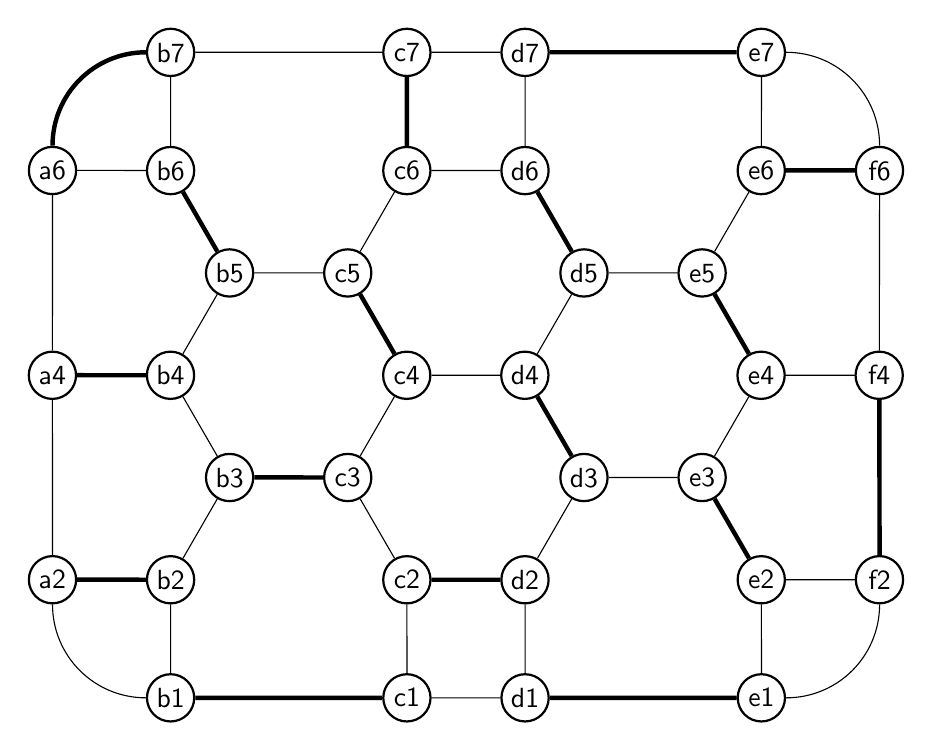
\begin{tikzpicture}[scale=1.5, bend angle=45, font=\sffamily]
          \foreach \n/\x in {a/1, b/2, c/4, d/5, e/7,f/8} {
            \node[v] (\n4) at (\x,4) {\n4};
          }
          \foreach \n in {b,d} {
            \node[v] (\n3) at ($(\n4) + (300:1)$) {\n3};
            \node[v] (\n5) at ($(\n4) + ( 60:1)$) {\n5};
            \node[v] (\n2) at ($(\n3) + (240:1)$) {\n2};
            \node[v] (\n6) at ($(\n5) + (120:1)$) {\n6};
            \node[v] (\n1) at ($(\n2) + (270:1)$) {\n1};
            \node[v] (\n7) at ($(\n6) + ( 90:1)$) {\n7};
          }
          \foreach \n in {c,e} {
            \node[v] (\n3) at ($(\n4) + (240:1)$) {\n3};
            \node[v] (\n5) at ($(\n4) + (120:1)$) {\n5};
            \node[v] (\n2) at ($(\n3) + (300:1)$) {\n2};
            \node[v] (\n6) at ($(\n5) + ( 60:1)$) {\n6};
            \node[v] (\n1) at ($(\n2) + (270:1)$) {\n1};
            \node[v] (\n7) at ($(\n6) + ( 90:1)$) {\n7};
          }
          \foreach \h in {2,6} {
            \node[v] (a\h) at ($(b\h) + (180:1)$) {a\h};
            \node[v] (f\h) at ($(e\h) + (  0:1)$) {f\h};
          }
          \draw[ultra thick] (b7) to[bend right] (a6);
          \draw (a2) to[bend right] (b1)
                (e1) to[bend right] (f2);
          \draw[ultra thick] (c2)--(d2)  (d1)--(e1)  (b3)--(c3)  (e2)--(e3)
                 (a4)--(b4)  (c4)--(c5)  (d3)--(d4)  (e4)--(e5)
                 (b5)--(b6)  (c6)--(c7)  (d5)--(d6)  (d7)--(e7) (a2)--(b2) 
                 (b1)--(c1) (f2)--(f4) (e6)--(f6);
          \draw (f6) to[bend right] (e7);
          \draw (b2)--(b3)--(b4)--(b5)--(c5)--(c6)--(d6)--(d7)--(c7)--(b7)--(b6)
              --(a6)--(a4)--(a2) (b2)--(b1) (c1)--(d1)--(e1)--(e2)--(f2) (f4)
              --(e4)--(e3)--(d3)--(d2)--(c2)--(c3)--(c4)--(d4)--(d5)--(e5)--(e6)
              --(f6)  (e6)--(e7) (c1)--(c2) (d2)--(d1) (f4)--(f6);
        \end{tikzpicture}
      \end{center}
\end{center}

This is the graph resulting from augmenting the matching along the path. Since there are no more M-unsaturated vertices the algorithm is stopped. The current matching is the maximum one.



 %%%%%%%%%%%%%%%%%%%%%%%%%%%%%%%%%%%%%%%%%%%%%%%%%%%%%%%%%%%%%%%%%%%%%%%%%%%%%%%%%%%%
%     Reference:
% \begin{center}
% \begin{tikzpicture}
%     [level distance=10mm,
%     % every node/.style={fill=red!60,circle,inner sep=1pt},
%     %,nodes={fill=red!30}
%     level 1/.style={sibling distance=40mm},
%     level 2/.style={sibling distance=20mm},
%     level 3/.style={sibling distance=11mm}]
%     \node[t]  {31} [grow=up]
%     %[sibling distance=0.7cm,level distance = 1.4cm,red]
%     child[draw=black, thin] { 
%         node[t] {30}
%         child[draw=black, ultra thick] { 
%             node[t] {20}
%             child[draw=black, thin] {
%                 node[t] {5}
%                 }
%             child[draw=black, thin] {
%                 node[t] {4}
%             }
%         }
%         child[draw=black, ultra thick] {
%             node[t] {10}
%             child[draw=black, thin] {
%                 node[t] {9}
%                 }
%             child[draw=black, thin] {
%                 node[t] {1}
%                 }
%             }
%     }
%     child [draw=black, thin] {
%         node[t] {20}
%         child[draw=black, ultra thick] {
%             node[t] {19}
%             child[draw=black, thin] {
%                 node[t] {1}
%                 }
%             child[missing]
%         }
%         child[draw=black, ultra thick] {
%             node[t] {18}
%             }
%     };
%     \end{tikzpicture}


%     \begin{tikzpicture}[level distance=15mm,
%         level 1/.style={sibling distance=8mm},
%         level 2/.style={sibling distance=20mm},
%         level 3/.style={sibling distance=15mm}]
%         \node[t]  {$\alpha$} [grow=up]
%         %[sibling distance=0.7cm,level distance = 1.4cm,red]
%         child[draw=black, thin] { 
%             node[t] (a4) {a4}
%             child[draw=black, ultra thick] {
%                 node[t] {b4}
%                 child[draw=black, thin] { 
%                     node[t] (b5) {b5}
%                 }
%                 child[draw=black, thin] { 
%                     node[t] (b3) {b3}
%                 }
%             }
%             child[missing]
%         }
%         child[missing]
%         child [draw=black, thin] {
%             node[t] (c1) {c1}
%             child[draw=black, ultra thick] {
%                 node[t] {c2}
%                 child[draw=black, thin] { 
%                     node[t] (c3) {c3}
%                 }
%                 child[draw=black, thin] { 
%                     node[t] (d2) {d2}
%                 }
%             }
%         }
%         child[missing]
%         child [draw=black, thin] {
%             node[t] {b3}
%             child[missing]
%             child[draw=black, ultra thick] {
%                 node[t] {c3}
%                 child[draw=black, thin] { 
%                     node[t] (c3) {c3}
%                 }
%                 child[draw=black, thin] { 
%                     node[t] (d2) {d2}
%                 }
%             }
%         };
%         \end{tikzpicture}

% \end{center}

\end{document}
